\documentclass[a4paper,12pt,french]{article}
\usepackage[margin=2cm]{geometry}
\usepackage[thinfonts]{uglix2}
\nouveaustyle

\begin{document}
\titre{Arborescences - Exercices}{NSI2}{2022} 

\begin{exercice}[ : Parcours d'une arborescence]
Voici une arborescence
\begin{center}
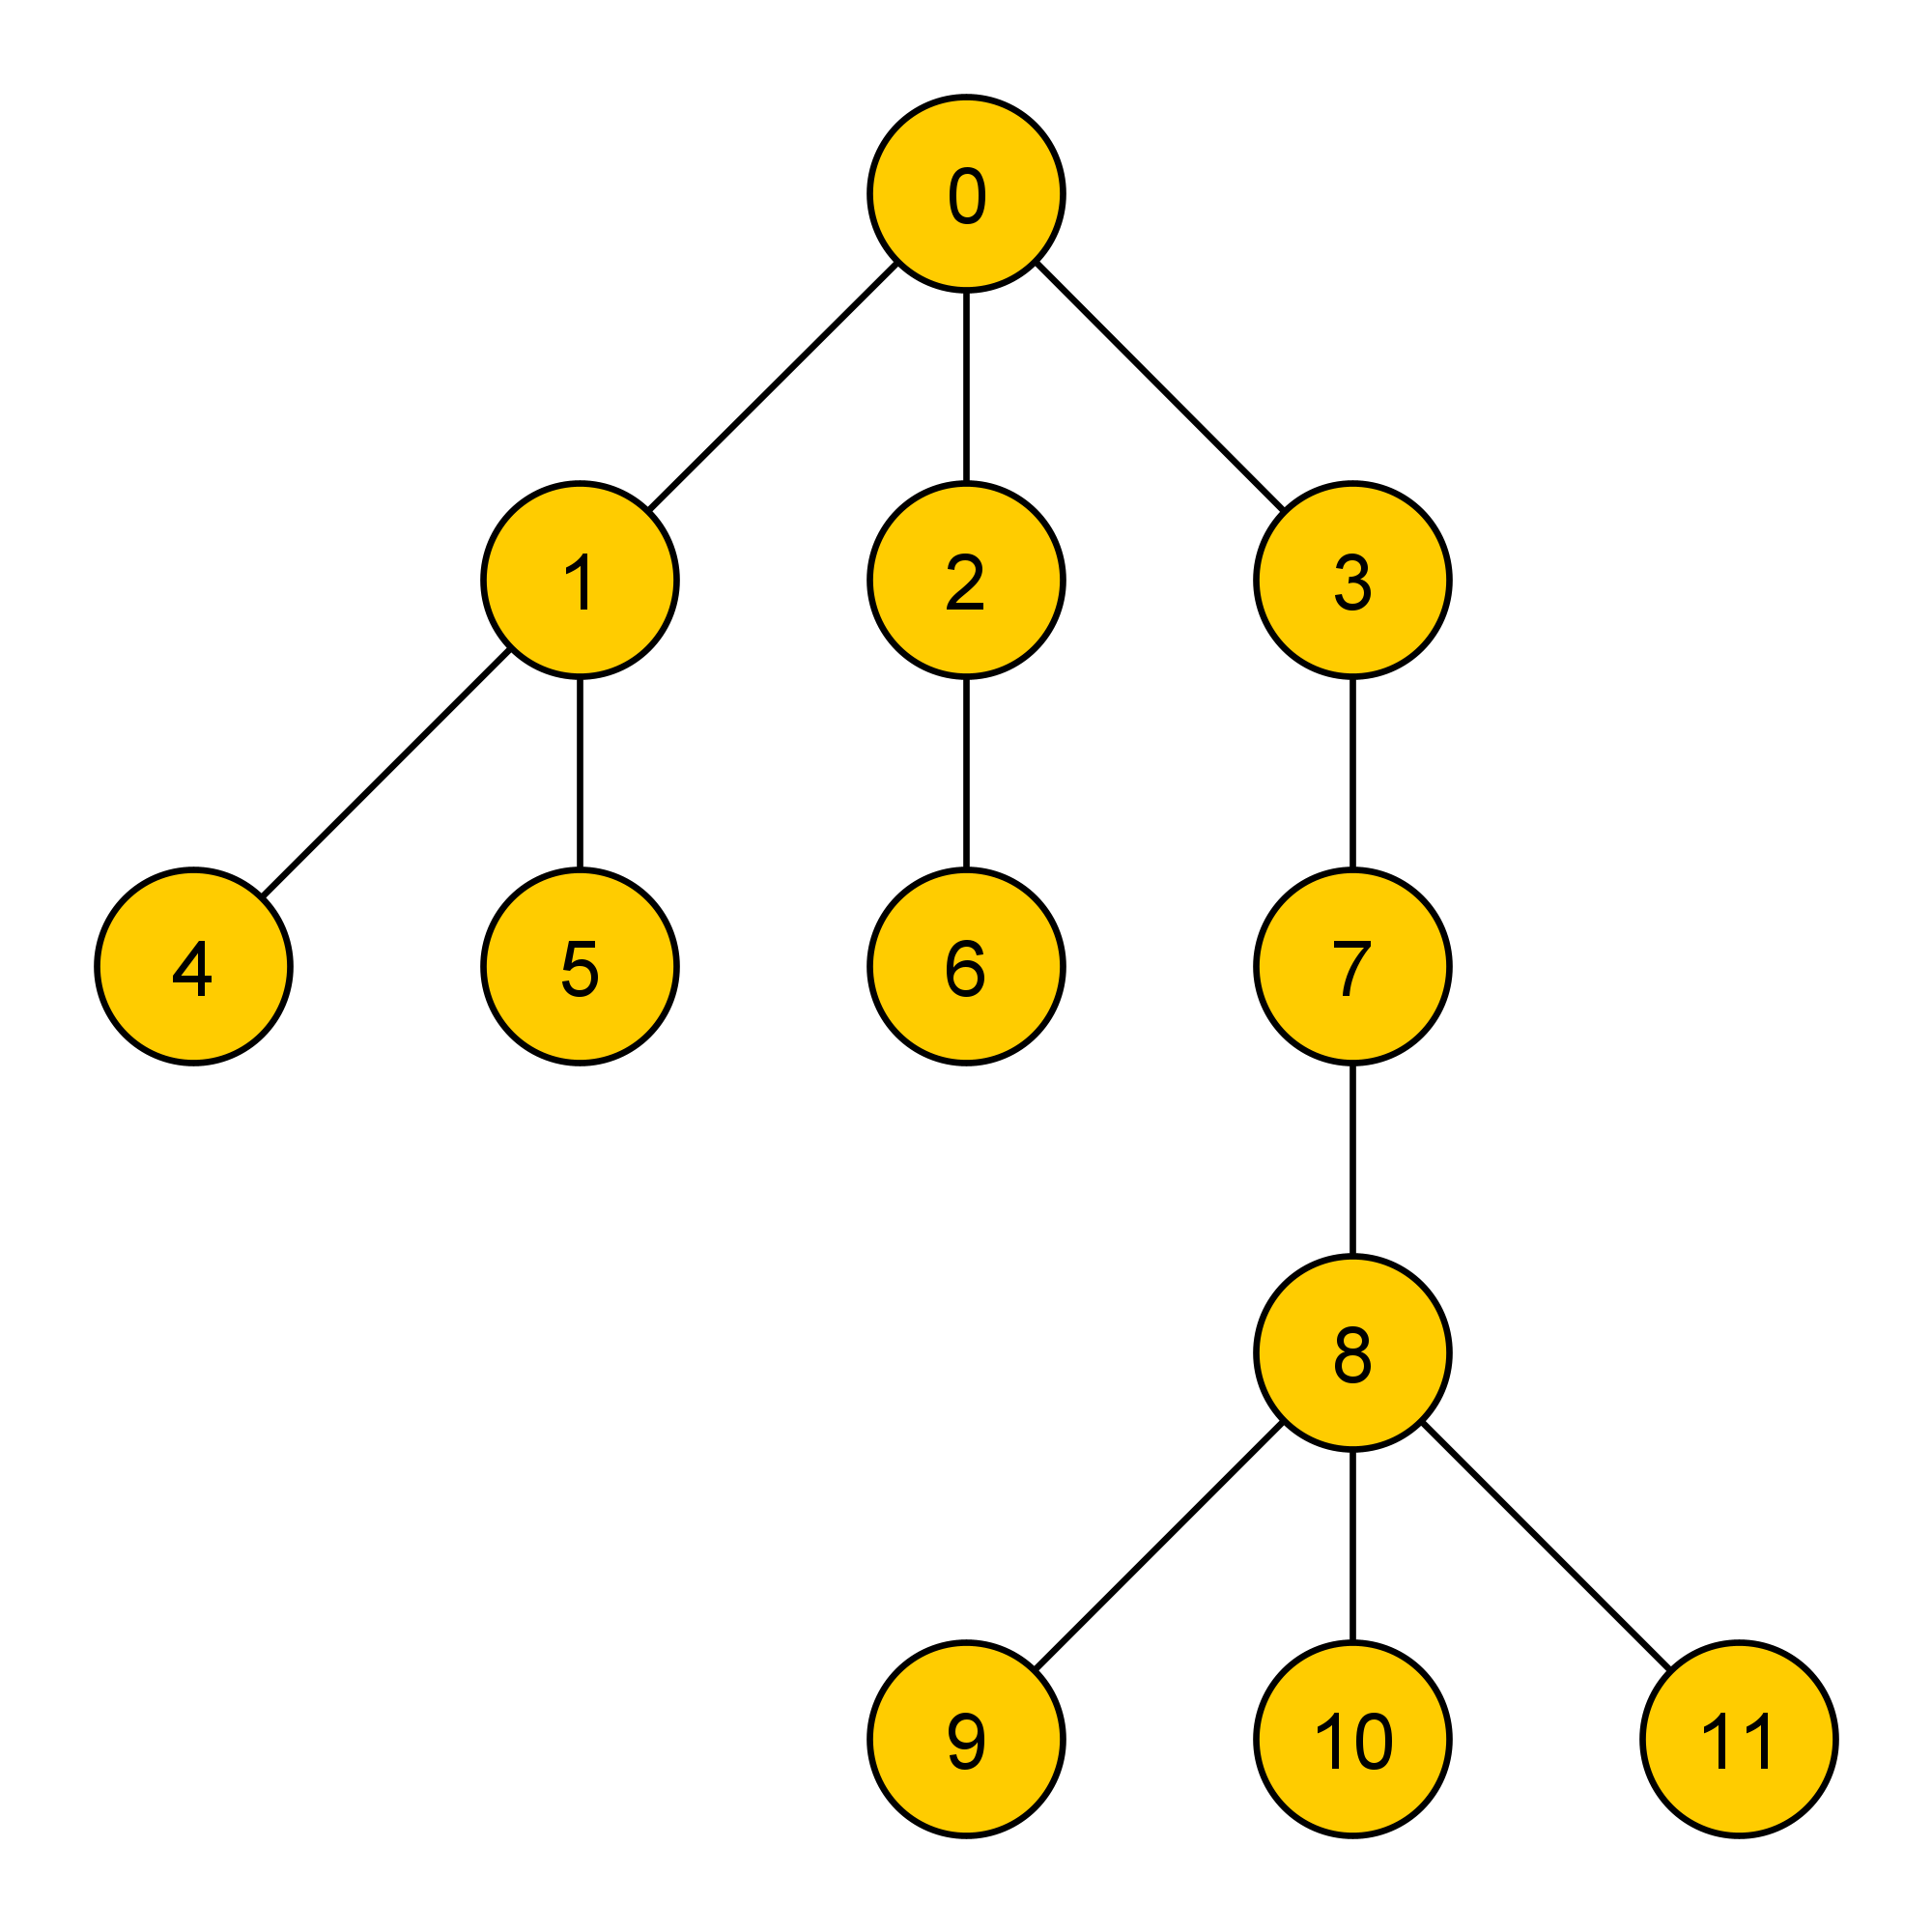
\includegraphics[width=7cm]{img/arbo1}
\end{center}
\begin{enumerate}[\bfseries 1.]
	\item 	Donner les valeurs des n\oe uds obtenues lors d'un parcours préfixe.
	\item 	Faire de même pour un parcours postfixe.
    \item 	Dans le fichier \texttt{nodeTS.py} se trouve une implémentation de cette arborescence.
    \begin{enumerate}[\bfseries a.]
    	\item 	Implémenter la méthode \texttt{prefixe} pour qu'elle affiche le parcours préfixe de l'arborescence (mettre un \pythoninline{print} dans cette méthode)
    	\item 	Faire de même avec la méthode \texttt{postfixe}.
	    \item 	Modifier ces deux méthodes pour qu'elles n'affichent plus simplement le parcours, mais renvoient la liste des éléments dans l'ordre du parcours. Pour ce faire vous pouvez utiliser une variable de classe \texttt{liste\_parcours} dans un premier temps.
        \item 	Faire la même chose, mais sans variable de classe. Penser qu'une méthode peut prendre des paramètres par défaut, et que \texttt{prefixe} peut nécessiter en paramètre la liste des n\oe uds déjà parcourus).
    \end{enumerate}
\end{enumerate}
\end{exercice}

\begin{exercice}[ : Trie]
Le mot trie vient de l'Anglais et est tiré du verbe \textit{to retrieve} (extraire). Il peut se prononcer comme le verbe \textit{to try}.\\
Nous allons nous en servir pour stocker tout les mots d'un (gros) dictionnaire.\\
\begin{center}
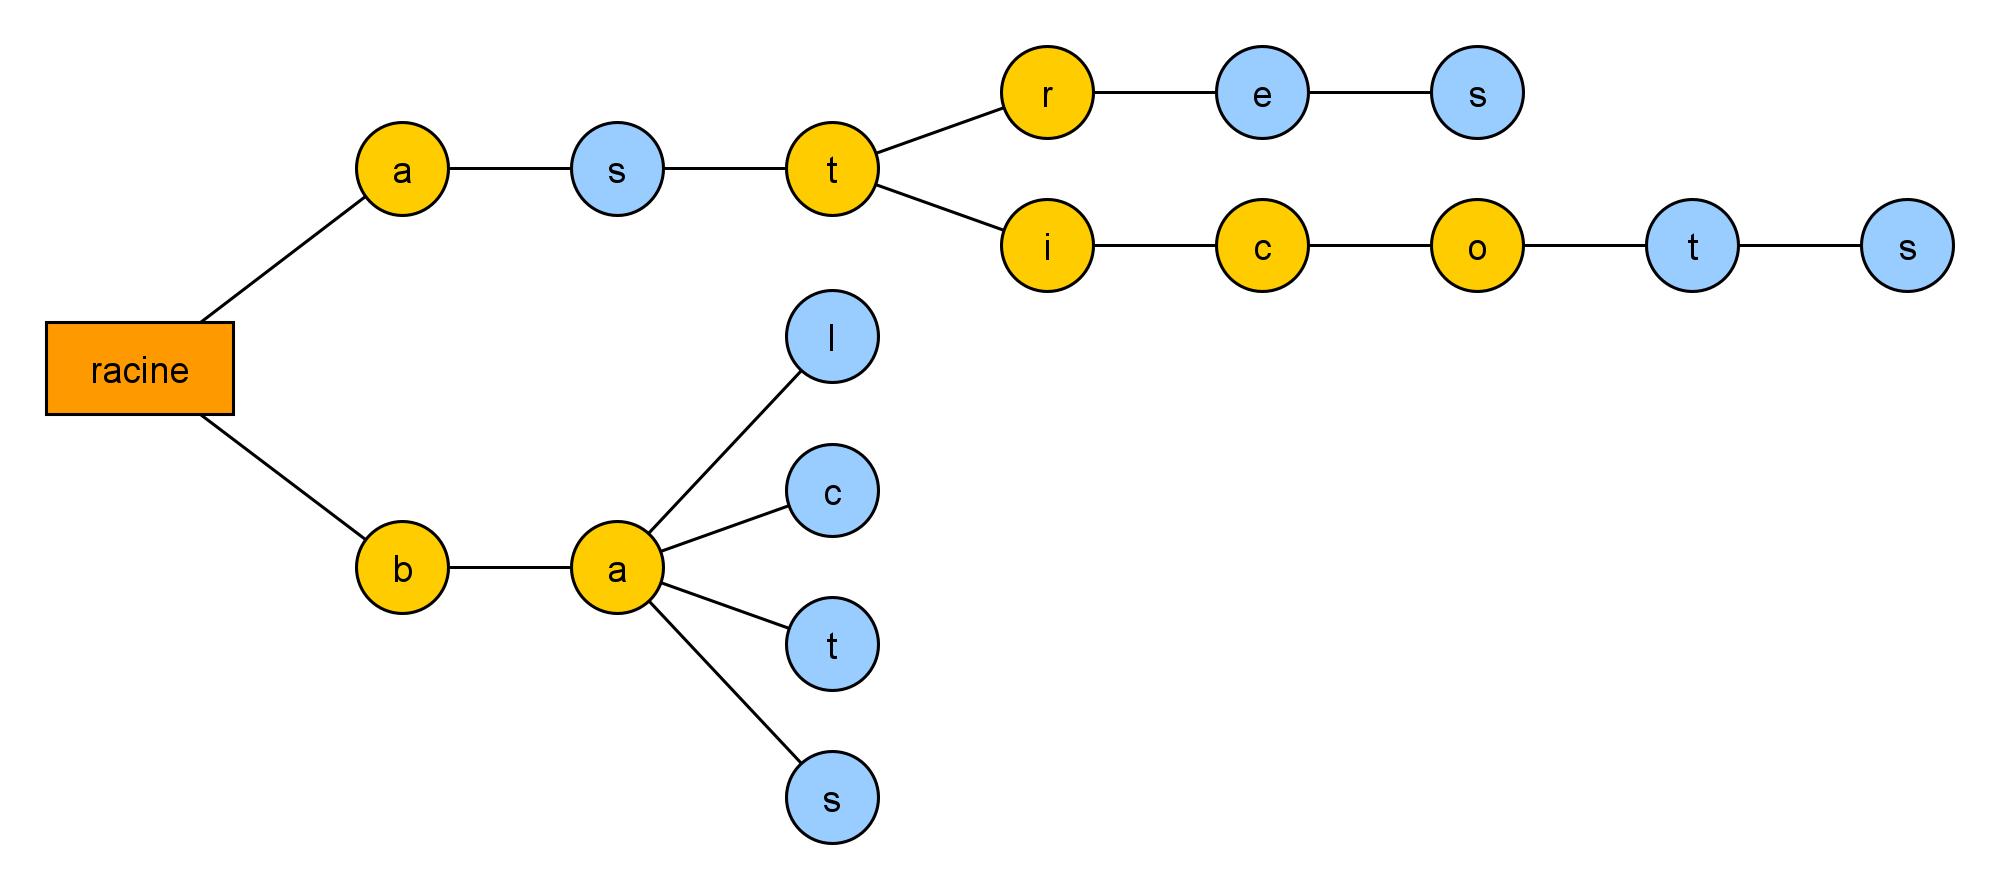
\includegraphics[width=10cm]{img/trie}
\end{center}
Le plus simple pour implémenter cette structure de données est de procéder ainsi : chaque n\oe ud contient
\begin{enumerate}[--]
	\item 	la lettre
	\item 	un booléen qui indique si oui ou non cette lettre termine un mot.
    \item 	un dictionnaire avec pour clés les lettres des fils du n\oe ud et pour valeur ces n\oe uds.
\end{enumerate}
\begin{minted}{python}
class NodeTrie:
    def __init__(self, lettre=None, est_fin=False):
        self.lettre = lettre
        self.est_fin = est_fin
        self.fils = dict()
\end{minted}

Ainsi, pour parcourir les lettres des n\oe uds qui sont les fils d'un n\oe ud donné (noté \pythoninline{self}), il suffit d'exécuter\\ \pythoninline{for lettre in self.fils}.\\

Pour parcourir effectivement les ,n\oe uds  on écrira\\ \pythoninline{for noeud in self.fils.values()}.\\

Pour créer la racine du trie, il suffit d'exécuter \pythoninline{racine = NodeTrie()}.
\begin{enumerate}[\bfseries 1.]
	\item 	\'Ecrire la méthode \texttt{ajoute\_ mot} qui
    \begin{enumerate}[--]
    	\item 	prend en entrée un mot qui est un \pythoninline{str};
    	\item 	ajoute ce mot à partir du n\oe ud courant.
    \end{enumerate}
    Dans les faits, l'utilisateur ne se  servira de cette méthode qu'à partir de la racine (mais pas le programmeur de cette méthode !).
    
    \item Pour peupler le trie avec les mots qui sont dans le fichier \texttt{dico.txt}, voici ce que vous devez écrire.
    
    \begin{minted}[fontsize=\scriptsize]{python}
with open('dico.txt', 'rt', encoding='utf8') as fichier:  # on ouvre le fichier
    ligne = fichier.readline()  # on lit une ligne
    while ligne: # tant que la ligne n'est pas vide
        trie.ajoute_mot(ligne[:-1])  # On enlève le dernier caractere, c'est un \n
        ligne = fichier.readline()  # On passe au mot suivant
    \end{minted}
    
    Ce fichier contient presque tous les mots de la langue française, en majuscules et sans accents. 
	\item 	\'Ecrire la méthode \texttt{contient} qui
  \begin{enumerate}[--]
    	\item 	prend en entrée un mot qui est un \pythoninline{str};
    	\item 	renvoie \pythoninline{True} si ce mot appartient à l'arborescence qui part du n\oe ud et \texttt{False} sinon.
    \end{enumerate}
    Là encore l'utilisateur n'utilisera cette méthode qu'à partir de la racine (mais pas le programmeur de cette méthode !).
    \item tester la méthode sur le trie.
    \item (facultatif) écrire une méthode \texttt{commence\_par} qui :
     \begin{enumerate}[--]
     	\item 	en entrée prend un début de mot qui est un \pythoninline{str};
     	\item 	renvoie la liste de tous les mots qui commencent par ce	début s'il y en a.
     \end{enumerate}
\end{enumerate}
\end{exercice}

\end{document}